\section{溶液物性および圧力場の確認}
\subsection{粘度計測}
鋼球落下実験を行う試験溶液として,1wt.\%PAA溶液の製作を行った.この製作した溶液の粘度特性を確認し,先行研究\cite{ref:9}\cite{ref:10}における粘度特性と比較した.なお,溶媒中の溶質が不均一であったり,混合時に混入する気泡が存在すると,溶液の粘度が正しく計測できない.十分な溶質拡散や脱泡のために時間を要するため,粘度計測は溶液作製直後ではなく,1週間後に行った.それぞれの試料に対し,円錐回転子の回転数を変化させ,各5回計測を行いその平均を求めた.

水道水の粘度計測結果をFig.\ref{fig:water-vis}に示す.なお,縦軸は粘度,横軸はせん断速度を表す.第2.2節においても示したが,コーンロータの回転速度に応じて,液体のせん断速度を変化させた.その結果,粘度は約1.1[mPa$\cdot$ s]でほぼ一定となっていた.これは,水がニュートン流体であり,粘度を比例係数とした速度勾配とせん断応力の比例関係となっているためであると考えられる.

水道水の場合と同様にPAA溶液の粘度計測を行った結果をFig.\ref{fig:PAA-vis}に示す.なお,縦軸は粘度の対数,横軸はせん断速度の対数を表す.また,Iwamuro {\it et al.}\cite{ref:9}やShiratori {\it et al.}\cite{ref:10}の文献値も共に示した.ここで,粘度$\mu$はせん断速度$\dot{\gamma}$に対して,粘度定数 k[Pa$\cdot$ $\text{s}^n$],指数$n$を用い Power-law modelに従うものとすると,
\begin{eqnarray}
    \label{eq:power-low}
    \mu=k\cdot\dot{\gamma}^{n-1}
\end{eqnarray}
といった式で与えられる\cite{ref:1}.式(\ref{eq:power-low})を用いて近似線計算を行った結果を,Table \ref{table:power-law}に示す.今回作製したPAA溶液は,Iwamuro {\it et al.}と比較し,Shear-thinning性が強く,粘度は弱いかった.またShiratori {\it et al.}と比較すると,Shear-thinning性は弱く,粘度は強い溶液であった.

\begin{figure}[ht]
    \centering
    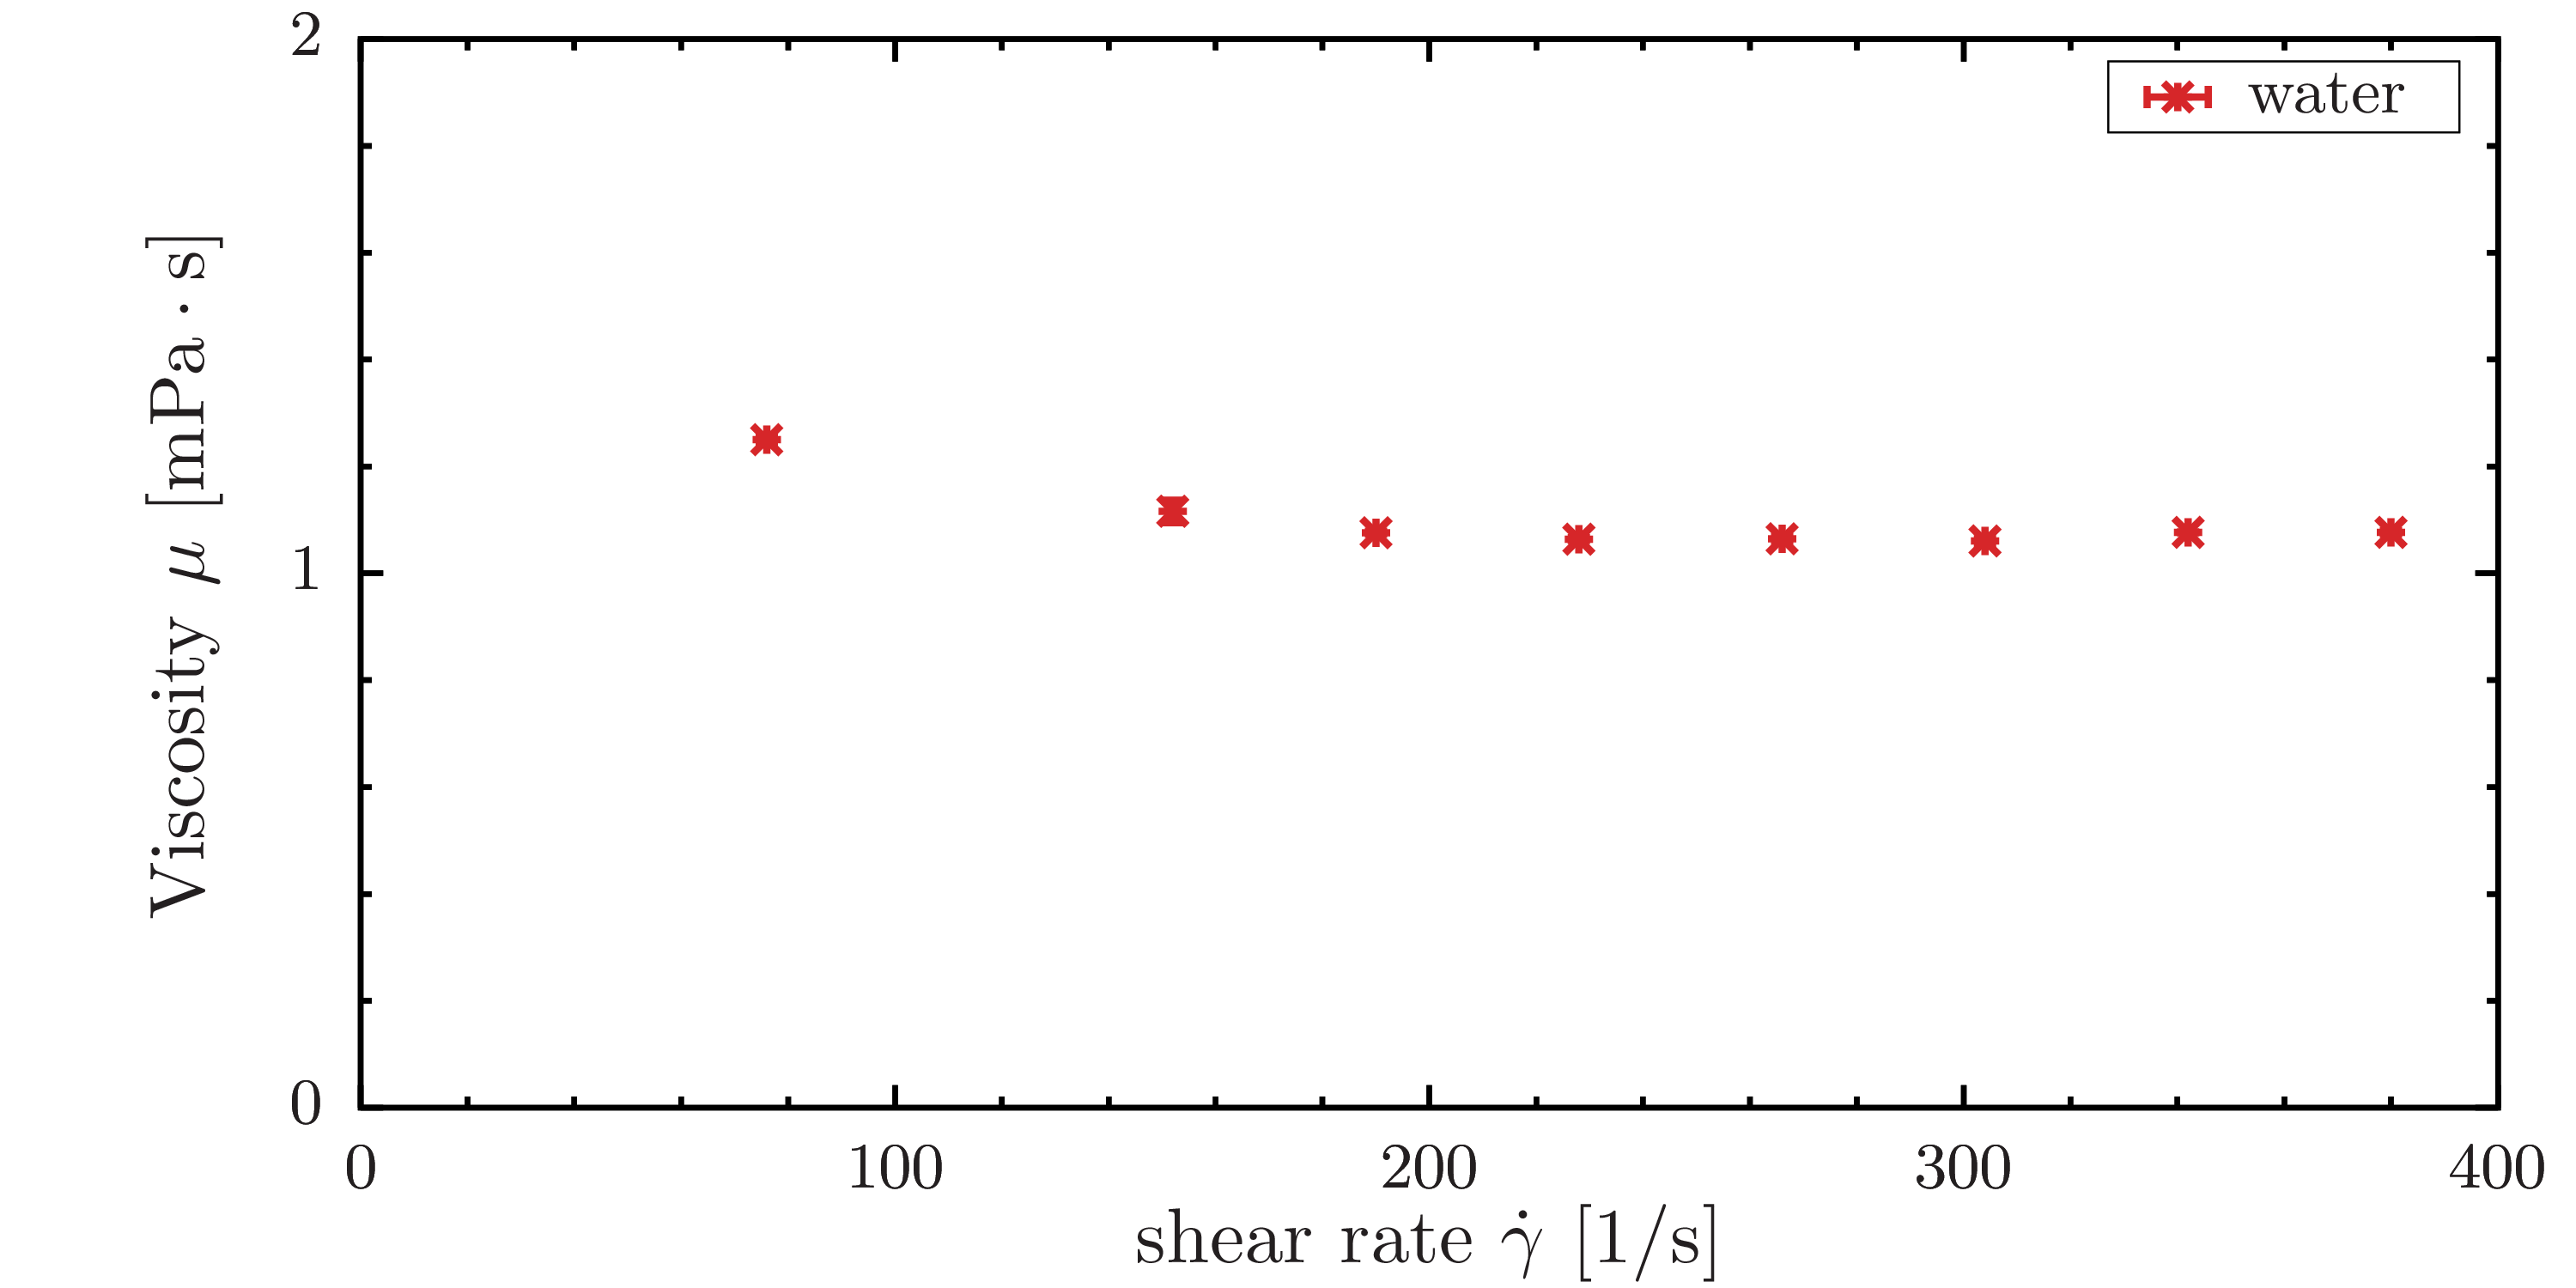
\includegraphics[width=12cm,clip]{4-Results/water.png}
    \caption{Meansured viscosity versus shear rate for tap water.}
    \label{fig:water-vis}
\end{figure}

\begin{figure}[ht]
    \centering
    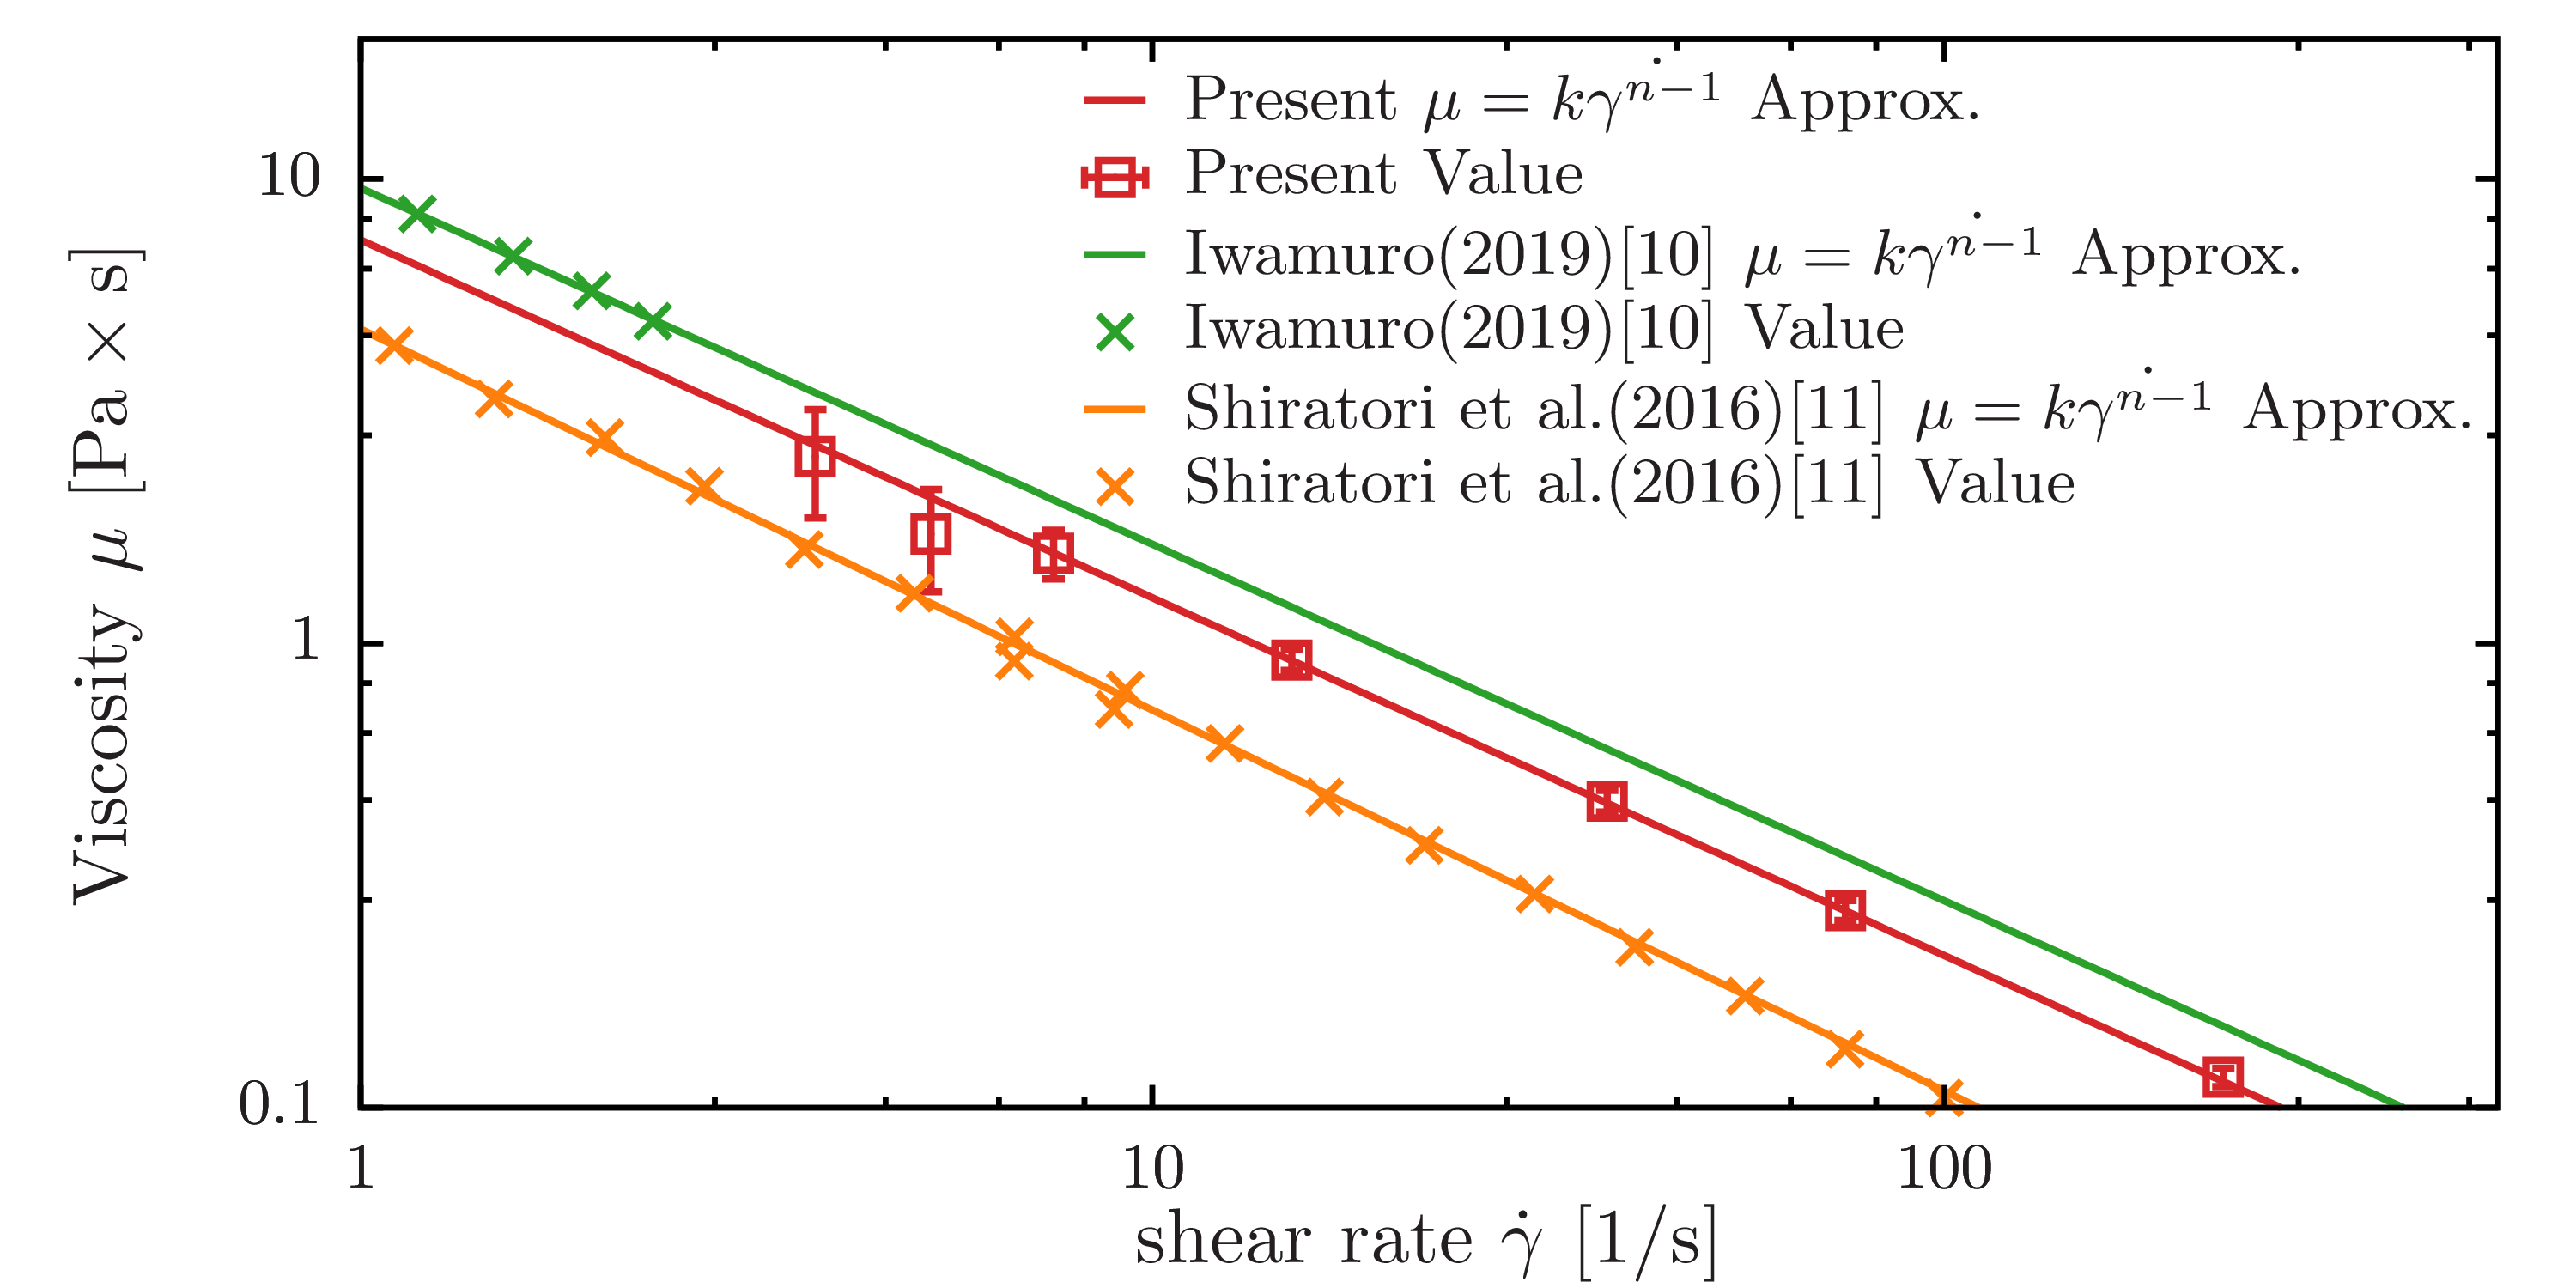
\includegraphics[width=13cm,clip]{4-Results/PAA-viscosity.png}
    \caption{Flow curve for 1wt.\%PAA solution.}
    \label{fig:PAA-vis}
\end{figure}

\begin{table}[h]
    \centering
    \caption{Parameters $k$ and $n$ in the power-law model for each experimental result.}
    \label{table:power-law}
    \begin{tabular}{c|c|c} \hline
        & k & n \\ \hline \hline
        Present & 8.37 & 0.24 \\
        Iwamuro\cite{ref:8} & 9.4 & 0.23 \\
        Shiratori \textit{et al}.(2016)\cite{ref:10} & 5.9 & 0.25 \\ \hline
    \end{tabular}
\end{table}

\newpage

\subsection{圧力振幅 計測結果}

容器A,Bそれぞれにおいて,超音波圧力振幅の計測を行った.容器Aにおける結果をFig.\ref{fig:pressure}(a),容器Bにおける結果をFig.\ref{fig:pressure}(b)に示す.縦軸は水槽底面からの高さ,横軸は圧力振幅である.この結果を元にTable \ref{table:press-A}, \ref{table:press-B} に,それぞれ,容器A,Bに対する圧力振幅$P$の$y$方向平均値を示す.どちらの水槽においても水槽全体に圧力振幅が発生していることが確認された.また,先行研究であるIwamuro\cite{ref:8}, Iwamuro \textit{et al}.\cite{ref:9}と同様な圧力振幅平均値となった.

\begin{table}[h]
    \centering
    \caption{Averaged value of pressure amplitude in tank A.}
    \label{table:press-A}
    \begin{tabular}{c|c|c}\hline
                       & Present 1wt.\% PAA & Iwamuro {\it et al.}\cite{ref:8} \\ \hline
        $\bar{P}$[kPa] &       68        & 72                              \\ \hline
    \end{tabular}
\end{table}

\begin{table}[h]
    \centering
    \caption{Averaged value of pressure amplitude in tank B.}
    \label{table:press-B}
    \begin{tabular}{c|c|c}\hline
                       & Present 1wt.\% PAA & Iwamuro \cite{ref:9} \\ \hline
        $\bar{P}$[kPa] & 159.2              & 180                              \\ \hline
    \end{tabular}
\end{table}

\begin{figure}[ht]
    \centering
    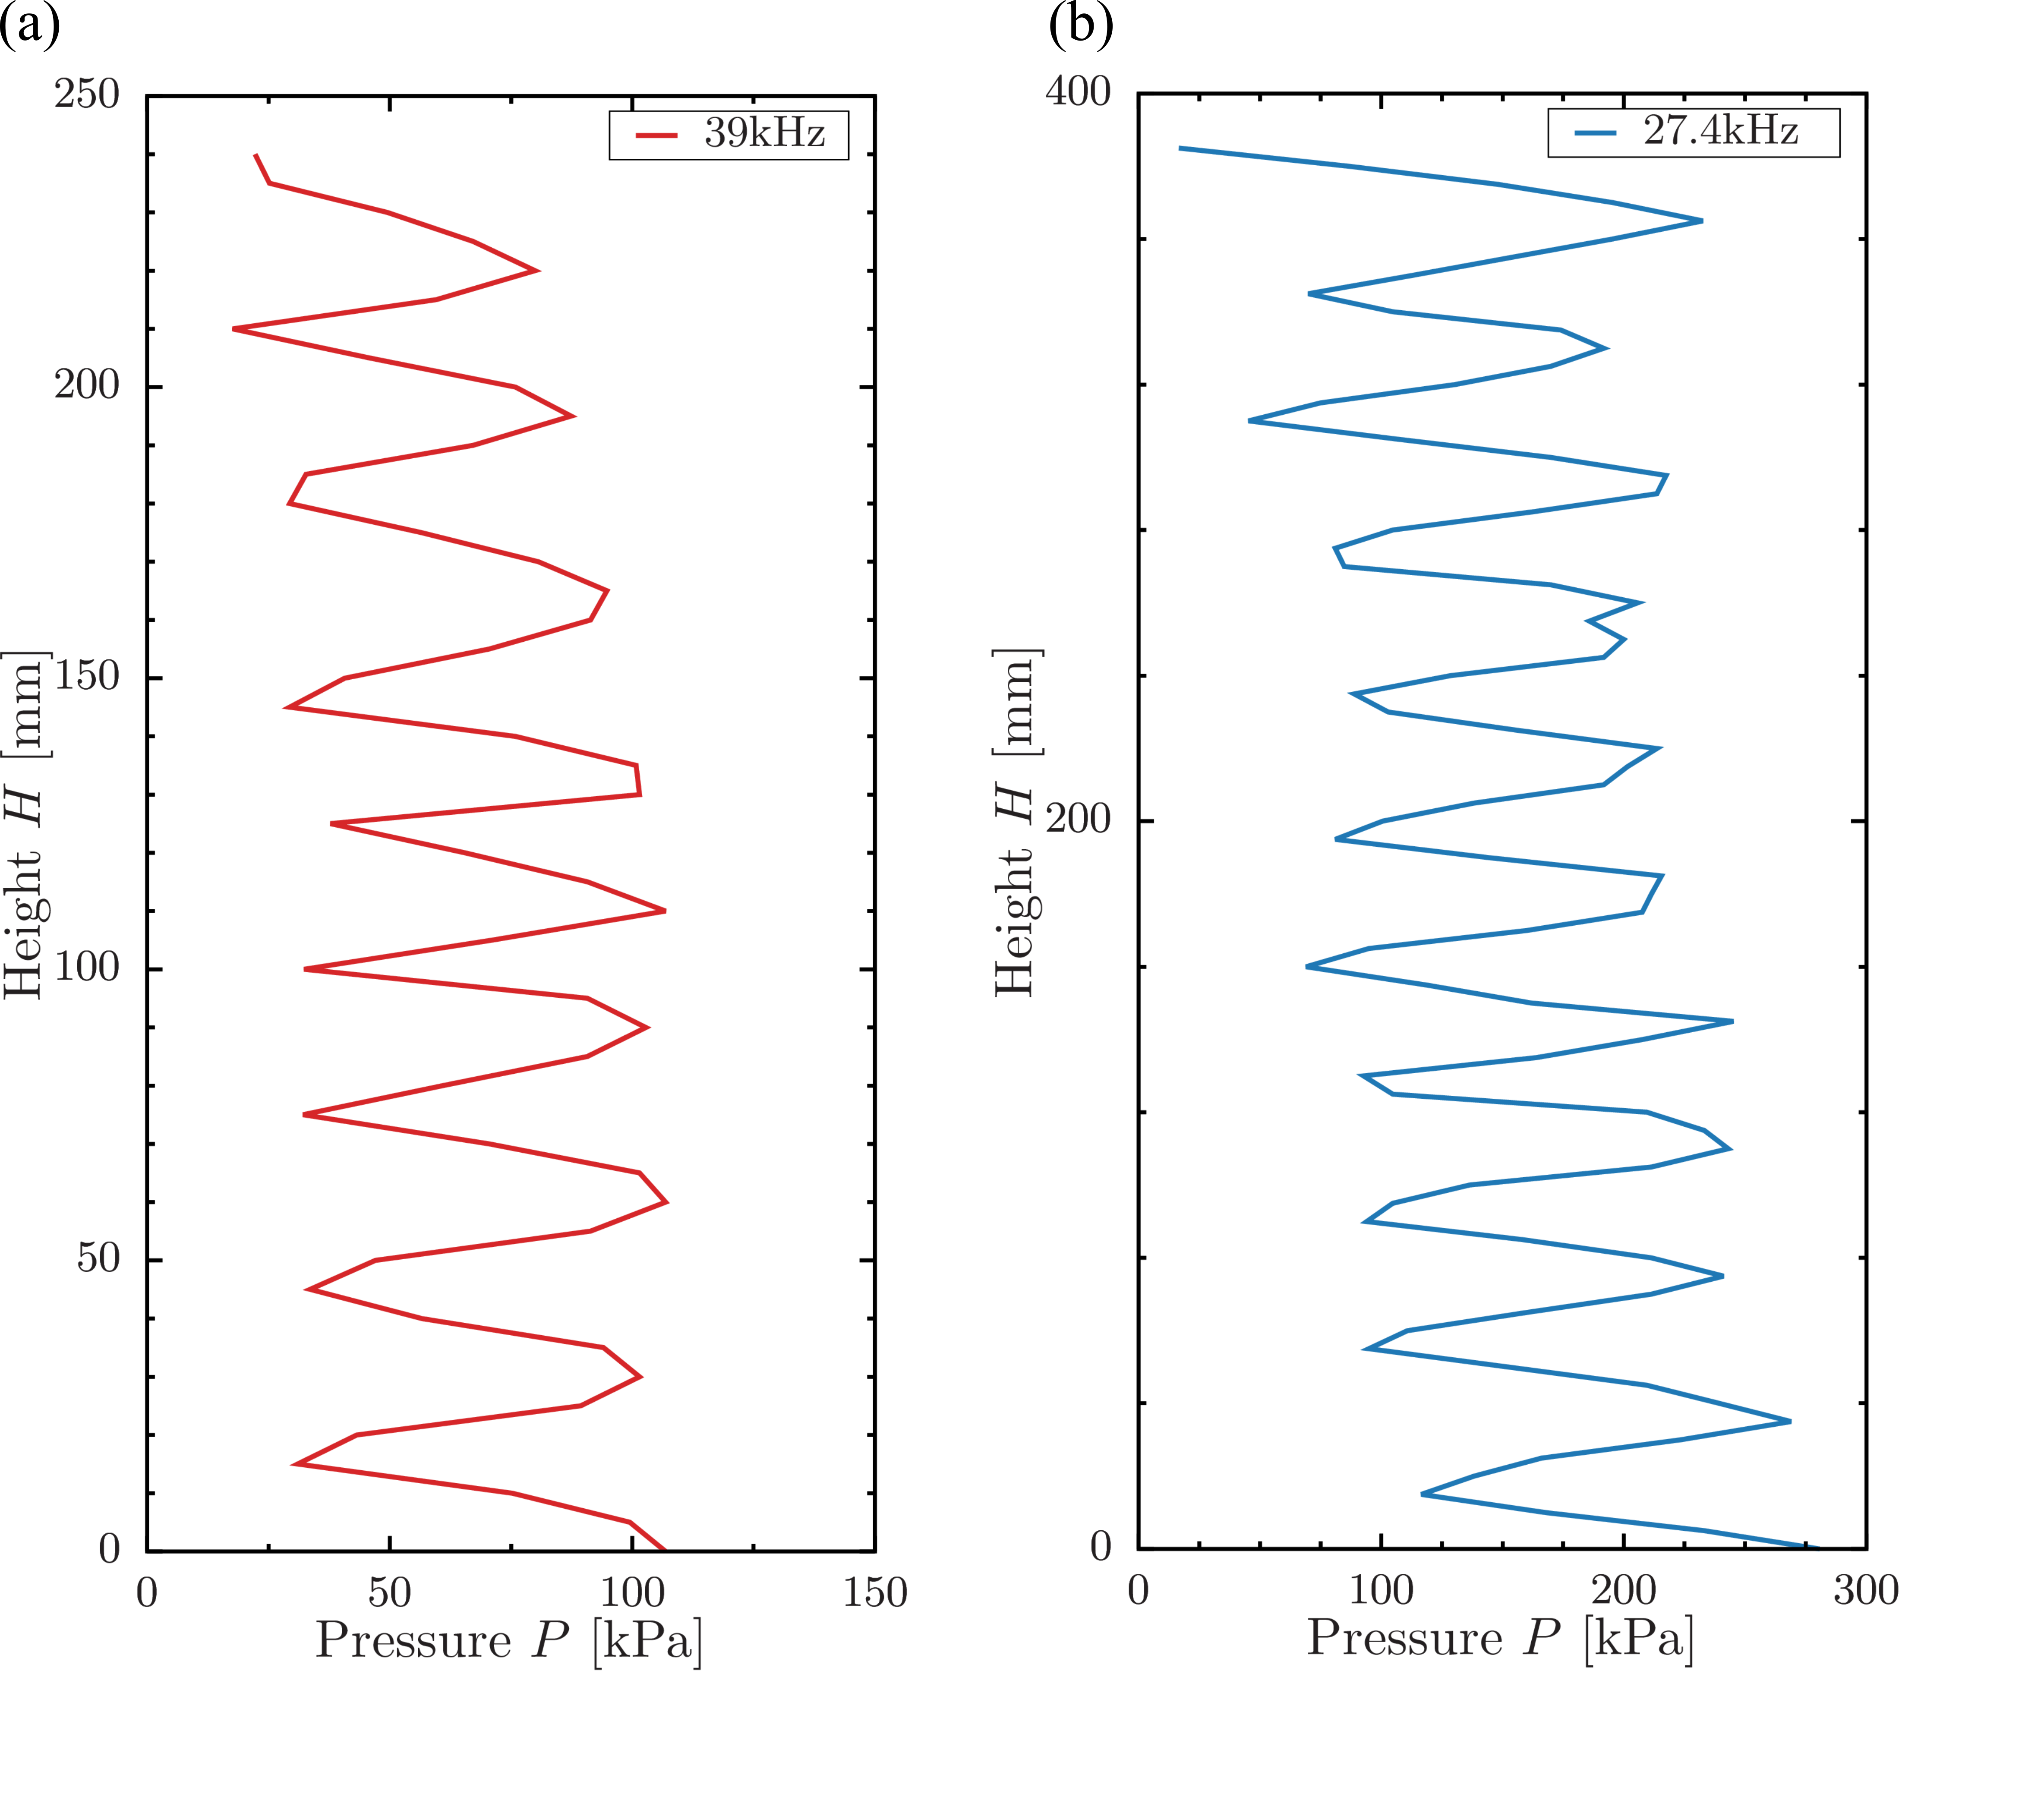
\includegraphics[width=12cm,clip]{4-Results/press.png}
    \caption{Average pressure amplitude in PAA solution. (a)In tank A. (b)In tank B.}
    \label{fig:pressure}
\end{figure}
